\documentclass[
  shownotes,
  xcolor={svgnames},
  hyperref={colorlinks,citecolor=DarkBlue,linkcolor=andesred,urlcolor=DarkBlue}
  , aspectratio=169]{beamer}
\usepackage{animate}
\usepackage{amsmath}
\usepackage{amsfonts}
\usepackage{amssymb}
\usepackage{pifont}
\usepackage{mathpazo}
%\usepackage{xcolor}
\usepackage{multimedia}
\usepackage{fancybox}
\usepackage[para]{threeparttable}
\usepackage{multirow}
\setcounter{MaxMatrixCols}{30}
\usepackage{subcaption}
\usepackage{graphicx}
\usepackage{lscape}
\usepackage[compatibility=false,font=small]{caption}
\usepackage{booktabs}
\usepackage{ragged2e}
\usepackage{chronosys}
\usepackage{appendixnumberbeamer}
\usepackage{animate}
\setbeamertemplate{caption}[numbered]
\usepackage{color}
%\usepackage{times}
\usepackage{tikz}
\usetikzlibrary{arrows}
\usepackage{comment} %to comment
%% BibTeX settings
\usepackage{natbib}
\bibliographystyle{apalike}
\bibpunct{(}{)}{,}{a}{,}{,}
\setbeamertemplate{bibliography item}{[\theenumiv]}

% Defines columns for bespoke tables
\usepackage{array}
\newcolumntype{L}[1]{>{\raggedright\let\newline\\\arraybackslash\hspace{0pt}}m{#1}}
\newcolumntype{C}[1]{>{\centering\let\newline\\\arraybackslash\hspace{0pt}}m{#1}}
\newcolumntype{R}[1]{>{\raggedleft\let\newline\\\arraybackslash\hspace{0pt}}m{#1}}


\usepackage{xfrac}


\usepackage{multicol}
\setlength{\columnsep}{0.5cm}

% Theme and colors
\usetheme{Boadilla}

% I define a custom pallete
\definecolor{andesred}{HTML}{1B175E}
\definecolor{andesyellow}{HTML}{ffff00}

% Other options
\providecommand{\U}[1]{\protect\rule{.1in}{.1in}}
\usefonttheme{serif}
\setbeamertemplate{itemize items}[default]
\setbeamertemplate{enumerate items}[square]
\setbeamertemplate{section in toc}[circle]


\definecolor{mybackground}{HTML}{1B175E}
\definecolor{myforeground}{HTML}{0000A0}

\setbeamercolor{normal text}{fg=black,bg=white}
\setbeamercolor{alerted text}{fg=andesred}
\setbeamercolor{example text}{fg=black}

\setbeamercolor{background canvas}{fg=myforeground, bg=white}
\setbeamercolor{background}{fg=myforeground, bg=mybackground}
\setbeamercolor{palette tertiary}{fg=myforeground,bg=mybackground}

\setbeamercolor{palette primary}{fg=black, bg=white}
\setbeamercolor{palette secondary}{fg=black, bg=white!10!andesyellow}
\setbeamercolor{palette tertiary}{fg=black, bg=white}


\setbeamercolor{frametitle}{fg=black}
\setbeamercolor{title}{fg=black}
\setbeamercolor{block title}{fg=andesred}
\setbeamercolor{itemize item}{fg=andesred}
\setbeamercolor{itemize subitem}{fg=andesred}
\setbeamercolor{itemize subsubitem}{fg=andesred}
\setbeamercolor{enumerate item}{fg=andesred}
\setbeamercolor{item projected}{bg=gray!30!white,fg=andesred}
\setbeamercolor{enumerate subitem}{fg=andesred}
\setbeamercolor{section number projected}{bg=gray!30!white,fg=andesred}
\setbeamercolor{section in toc}{fg=andesred}
\setbeamercolor{caption name}{fg=andesred}
\setbeamercolor{button}{bg=gray!30!white,fg=andesred}
\setbeamercolor{title in head/foot}{fg=andesred}



\usepackage{fancyvrb}
\newcommand{\VerbBar}{|}
\newcommand{\VERB}{\Verb[commandchars=\\\{\}]}
\DefineVerbatimEnvironment{Highlighting}{Verbatim}{commandchars=\\\{\}}
% Add ',fontsize=\small' for more characters per line
\usepackage{framed}
\definecolor{shadecolor}{RGB}{248,248,248}
\newenvironment{Shaded}{\begin{snugshade}}{\end{snugshade}}
\newcommand{\AlertTok}[1]{\textcolor[rgb]{0.94,0.16,0.16}{#1}}
\newcommand{\AnnotationTok}[1]{\textcolor[rgb]{0.56,0.35,0.01}{\textbf{\textit{#1}}}}
\newcommand{\AttributeTok}[1]{\textcolor[rgb]{0.77,0.63,0.00}{#1}}
\newcommand{\BaseNTok}[1]{\textcolor[rgb]{0.00,0.00,0.81}{#1}}
\newcommand{\BuiltInTok}[1]{#1}
\newcommand{\CharTok}[1]{\textcolor[rgb]{0.31,0.60,0.02}{#1}}
\newcommand{\CommentTok}[1]{\textcolor[rgb]{0.56,0.35,0.01}{\textit{#1}}}
\newcommand{\CommentVarTok}[1]{\textcolor[rgb]{0.56,0.35,0.01}{\textbf{\textit{#1}}}}
\newcommand{\ConstantTok}[1]{\textcolor[rgb]{0.00,0.00,0.00}{#1}}
\newcommand{\ControlFlowTok}[1]{\textcolor[rgb]{0.13,0.29,0.53}{\textbf{#1}}}
\newcommand{\DataTypeTok}[1]{\textcolor[rgb]{0.13,0.29,0.53}{#1}}
\newcommand{\DecValTok}[1]{\textcolor[rgb]{0.00,0.00,0.81}{#1}}
\newcommand{\DocumentationTok}[1]{\textcolor[rgb]{0.56,0.35,0.01}{\textbf{\textit{#1}}}}
\newcommand{\ErrorTok}[1]{\textcolor[rgb]{0.64,0.00,0.00}{\textbf{#1}}}
\newcommand{\ExtensionTok}[1]{#1}
\newcommand{\FloatTok}[1]{\textcolor[rgb]{0.00,0.00,0.81}{#1}}
\newcommand{\FunctionTok}[1]{\textcolor[rgb]{0.00,0.00,0.00}{#1}}
\newcommand{\ImportTok}[1]{#1}
\newcommand{\InformationTok}[1]{\textcolor[rgb]{0.56,0.35,0.01}{\textbf{\textit{#1}}}}
\newcommand{\KeywordTok}[1]{\textcolor[rgb]{0.13,0.29,0.53}{\textbf{#1}}}
\newcommand{\NormalTok}[1]{#1}
\newcommand{\OperatorTok}[1]{\textcolor[rgb]{0.81,0.36,0.00}{\textbf{#1}}}
\newcommand{\OtherTok}[1]{\textcolor[rgb]{0.56,0.35,0.01}{#1}}
\newcommand{\PreprocessorTok}[1]{\textcolor[rgb]{0.56,0.35,0.01}{\textit{#1}}}
\newcommand{\RegionMarkerTok}[1]{#1}
\newcommand{\SpecialCharTok}[1]{\textcolor[rgb]{0.00,0.00,0.00}{#1}}
\newcommand{\SpecialStringTok}[1]{\textcolor[rgb]{0.31,0.60,0.02}{#1}}
\newcommand{\StringTok}[1]{\textcolor[rgb]{0.31,0.60,0.02}{#1}}
\newcommand{\VariableTok}[1]{\textcolor[rgb]{0.00,0.00,0.00}{#1}}
\newcommand{\VerbatimStringTok}[1]{\textcolor[rgb]{0.31,0.60,0.02}{#1}}
\newcommand{\WarningTok}[1]{\textcolor[rgb]{0.56,0.35,0.01}{\textbf{\textit{#1}}}}
\usepackage{graphicx}
\makeatletter

\makeatother


\AtBeginSection[]
{
    \begin{frame}
        \frametitle{Agenda}
        \tableofcontents[currentsection]
    \end{frame}
}



\AtBeginSubsection[]
{
    \begin{frame}
        \frametitle{Agenda}
        \tableofcontents[currentsubsection]
    \end{frame}
}





%%%%%%%%%%%%%%% BEGINS DOCUMENT %%%%%%%%%%%%%%%%%%



\begin{document}

\title{Classification (Cont.)}
\subtitle{Big Data y Machine Learning para Economía Aplicada}
\date{}

\author[Sarmiento-Barbieri]{Ignacio Sarmiento-Barbieri}
\institute[Uniandes]{Universidad de los Andes}


\begin{frame}[noframenumbering]
\maketitle
\end{frame}






%----------------------------------------------------------------------% 

\begin{frame}
\frametitle{Agenda}

\tableofcontents

\end{frame}



%----------------------------------------------------------------------%
\section{Recap}
%----------------------------------------------------------------------%
%----------------------------------------------------------------------%
\begin{frame}[fragile]
\frametitle{Recap}

\begin{itemize}
  \item We observe $(y_i,X_i)$ $i=1,\dots,n$
  \medskip
  \item Estimate Probabilities
  \begin{itemize}
  \item Logit

    \begin{align}
    p_i &=\frac{e^{X_i\beta}}{1+e^{X_i\beta}}
    \end{align}
    \item get $\beta$
  \end{itemize}


\item Prediction
 \begin{itemize}
  \item Logit, with the $\hat{\beta}$

    \begin{align}
\hat{p}_i &=\frac{e^{X_i\hat{\beta}}}{1+e^{X_i\hat{\beta}}}
\end{align}  
      
  \end{itemize}


\item Classification 

\begin{align}
\hat{Y}_i= 1[\hat{p}_i >c]
\end{align}
\end{itemize}
\end{frame}
%----------------------------------------------------------------------%
\begin{frame}[fragile]
\frametitle{Performance}


\begin{figure}[H] \centering
            \captionsetup{justification=centering}
              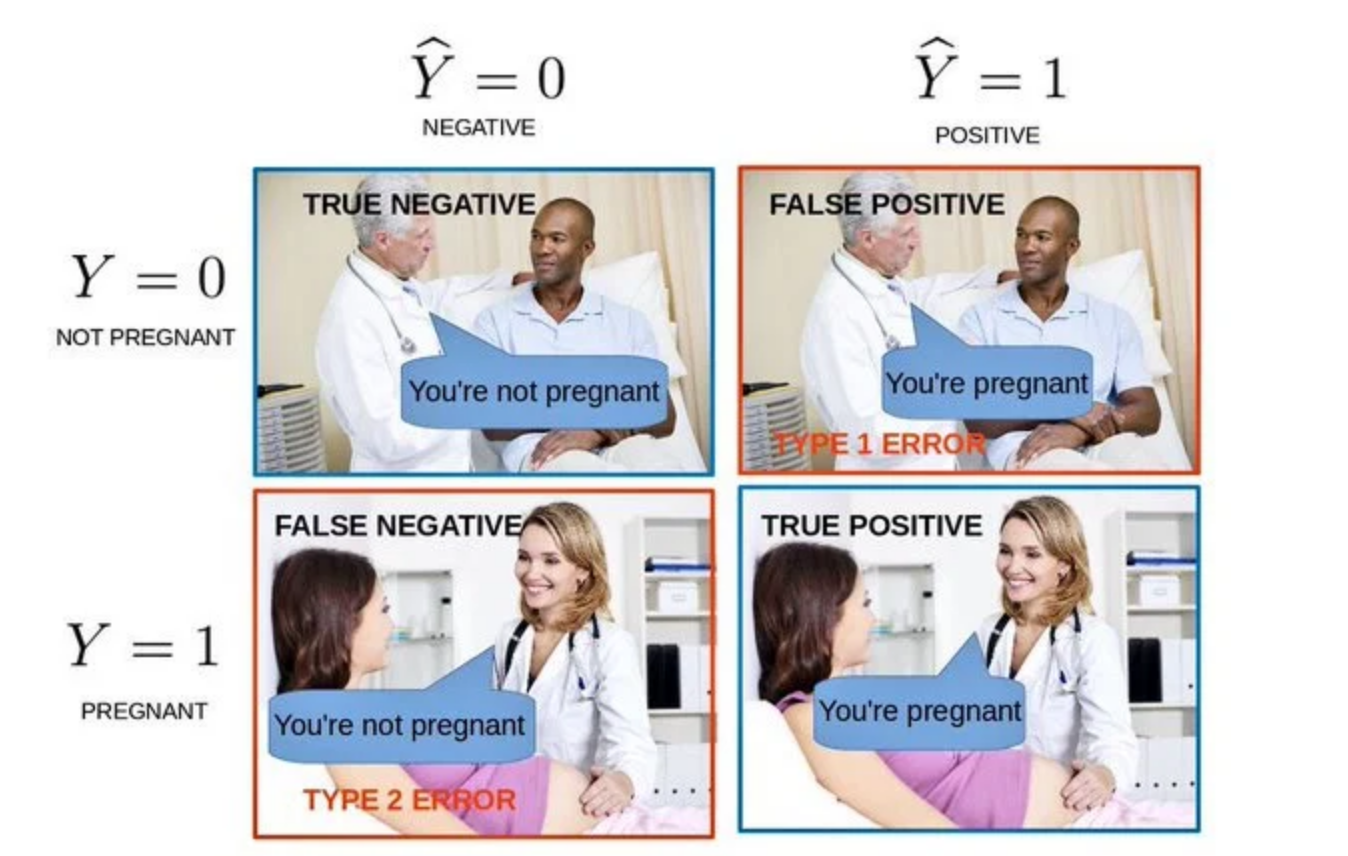
\includegraphics[scale=0.45]{figures/confusion_matrix}                            
 \end{figure}


\end{frame}
%----------------------------------------------------------------------%
\begin{frame}[fragile]
\frametitle{Performance}


 \begin{table}[]
\begin{tabular}{cccc}
                      &    & \multicolumn{2}{l}{$\hat{y}_i$} \\
                      &      & 0           & 1          \\
\multirow{2}{*}{$y_i$} & 0    & TN          & FP         \\
                      & 1    & FN          & TP        
\end{tabular}
\end{table}




\begin{itemize}

  \item We have two types of error associated with this that we can use as a measure of performance
  \medskip
  \begin{align}
     False\,Positive\,Rate&=\frac{False\,\,Positives}{Negatives} \nonumber \\
     True\,Positive\,Rate&=\frac{True \,\,Positives}{Positives} 
  \end{align}
  \item Another names they receive:
  \begin{itemize}
    \item False positive rate: Type I error, 1-Specificity
    \item True positive rate: 1- Type II error, power, sensitivity.
  \end{itemize}
\end{itemize}

\end{frame}

%----------------------------------------------------------------------%
\section{Other Models for Classification}
%----------------------------------------------------------------------%
\subsection{Regularization for Logit}
%----------------------------------------------------------------------%
\begin{frame}[fragile]
\frametitle{Regularization for Logit}

\begin{align}
\min_{\beta_0,\dots,\beta_k} \frac{1}{N} \sum_{i=1}^{N} l(y_i,\beta_0 + x_{i1}\beta_1 + \dots + x_{ik}\beta_k) + \lambda\left( \alpha \sum_{j=1}^k |\beta_j| + (1-\alpha)\ \sum_{j=1}^k (\beta_j)^2/2 \right)
\end{align}

\begin{itemize}
 \item Si $\alpha=1$ Lasso
 \medskip
 \item Si $\alpha=0$ Ridge 
\end{itemize}

\end{frame}
%----------------------------------------------------------------------%
\subsection{KNN}
%----------------------------------------------------------------------%
\begin{frame}[fragile]
\frametitle{K-Nearest Neighbors}

\begin{itemize}
\item K nearest neighbor (K-NN) algorithm predicts class $\hat y$ for $x$ by asking \\
{\it What is the most common class for observations around x?}
\end{itemize}
        \begin{figure}[H] \centering
            \captionsetup{justification=centering}
              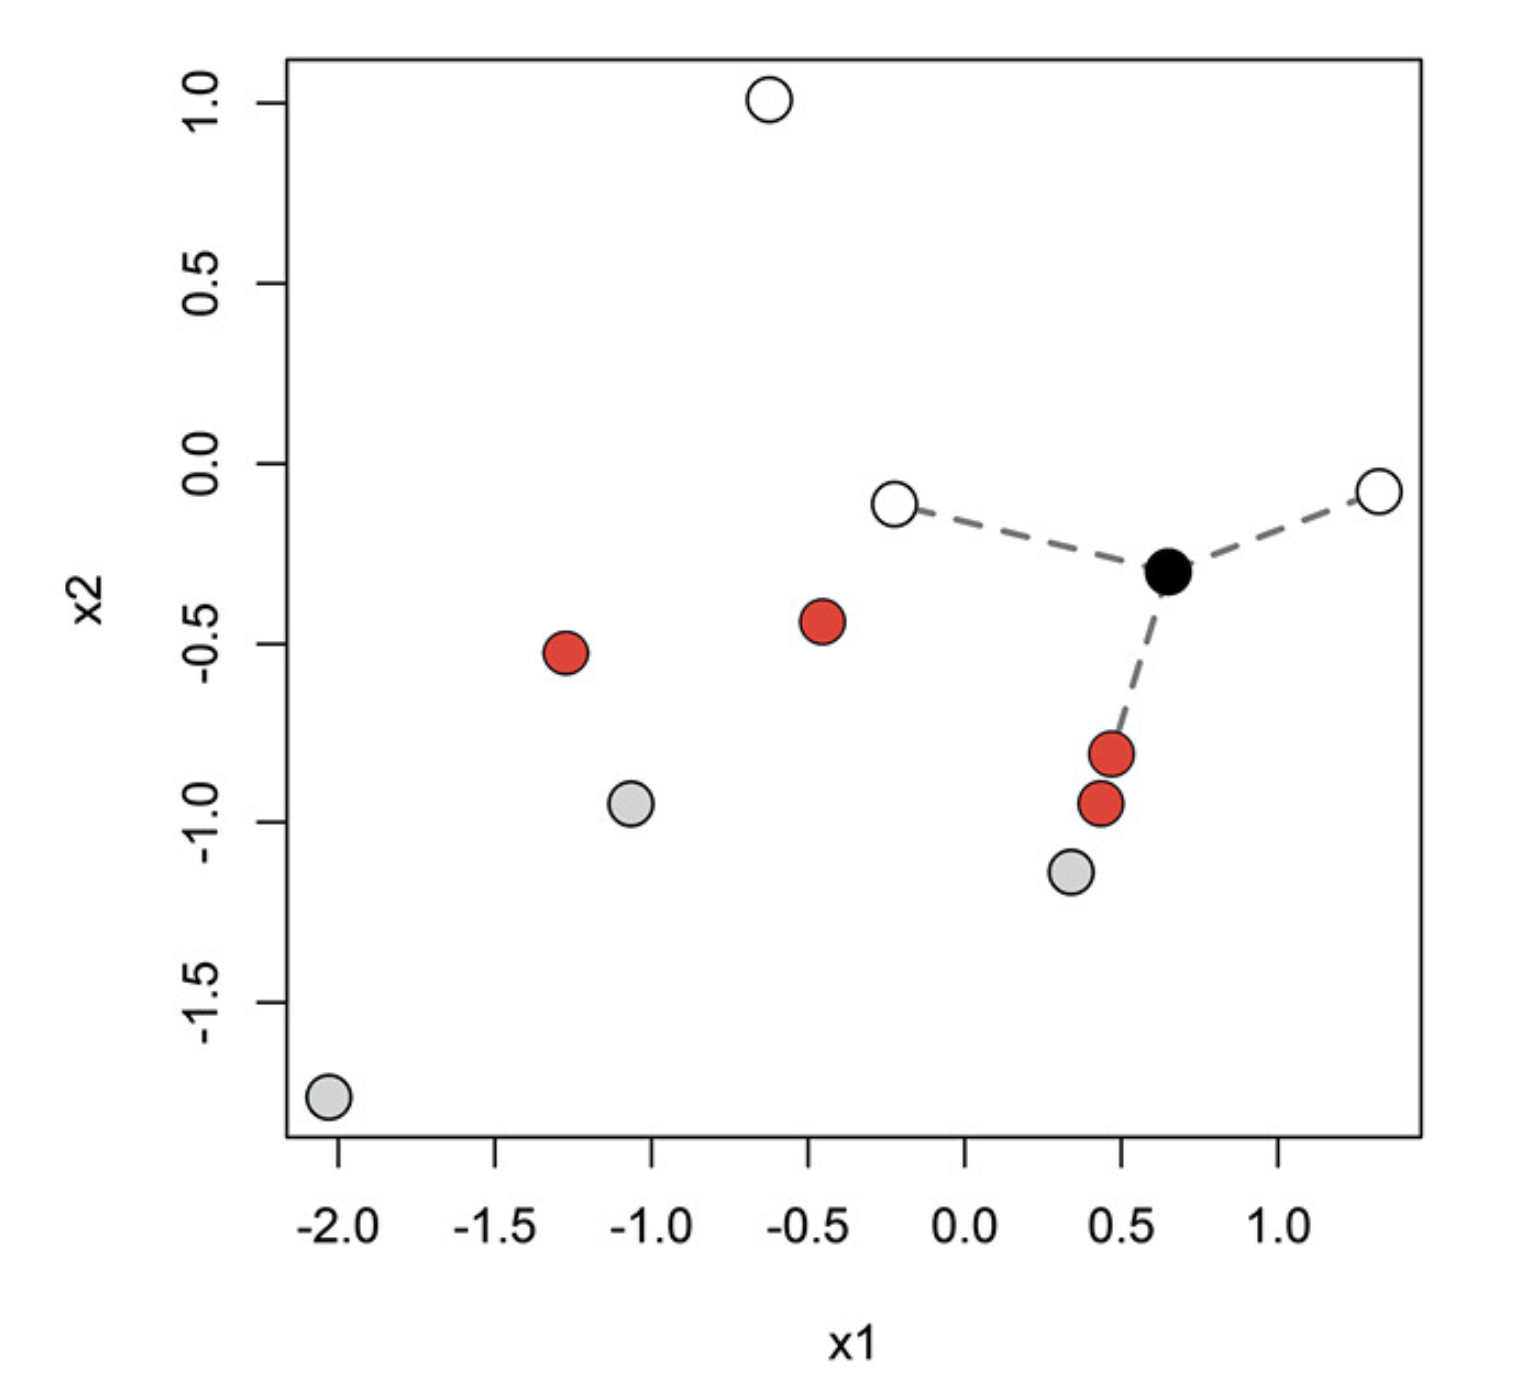
\includegraphics[scale=0.13]{figures/knn}
              \\
              \tiny
              Source: Taddy (2019)
 \end{figure}


 \end{frame}
%----------------------------------------------------------------------%
\begin{frame}[fragile]
\frametitle{K-Nearest Neighbors}

\begin{itemize}
\item K nearest neighbor (K-NN) algorithm predicts class $\hat y$ for $x$ by asking \\
{\it What is the most common class for observations around x?}
\item Algorithm: given an input vector $x_f$ where you would like to predict the class label

\begin{itemize}
  \item Find the K nearest neighbors in the dataset of labeled observations, $\{x_i,y_i\}_{i=1}^n$, the most common distance is the Euclidean distance:
  \begin{align}
  d(x_i,x_f)=\sqrt{\sum_{j=1}^p(x_{ij}-x_{fj})^2}
  \end{align}
  \item This yields a set of the $K$ nearest observations with labels: 
  \begin{align}
  [x_{i1},y_{i1}],\dots,[x_{iK},y_{iK}]
  \end{align}
  \item The predicted class of $x_f$ is the most common class in this set
  \begin{align}
  \hat{y}_f =mode\{y_{i1},\dots,y_{iK}\}
  \end{align}
\end{itemize}

\end{itemize}
\end{frame}


%----------------------------------------------------------------------%
\begin{frame}[fragile]
\frametitle{K-Nearest Neighbors}
\begin{itemize}
  \item There are some major problems with practical implications
  \medskip
  \begin{itemize}
  \item Knn predictions are unstable as a function of $K$
    \end{itemize}
\end{itemize}
  \begin{columns}[T] % align columns
\begin{column}{.58\textwidth}
\begin{align}
  K&=1 \implies \hat{p}(white)=0 \nonumber \\
  K&=2 \implies \hat{p}(white)=1/2 \nonumber \\
  K&=3 \implies \hat{p}(white)=2/3 \nonumber \\
  K&=4 \implies \hat{p}(white)=1/2 \nonumber 
  \end{align}


\end{column}
\hfill
\begin{column}{.4\textwidth}
\begin{figure}[H] \centering
            \captionsetup{justification=centering}
              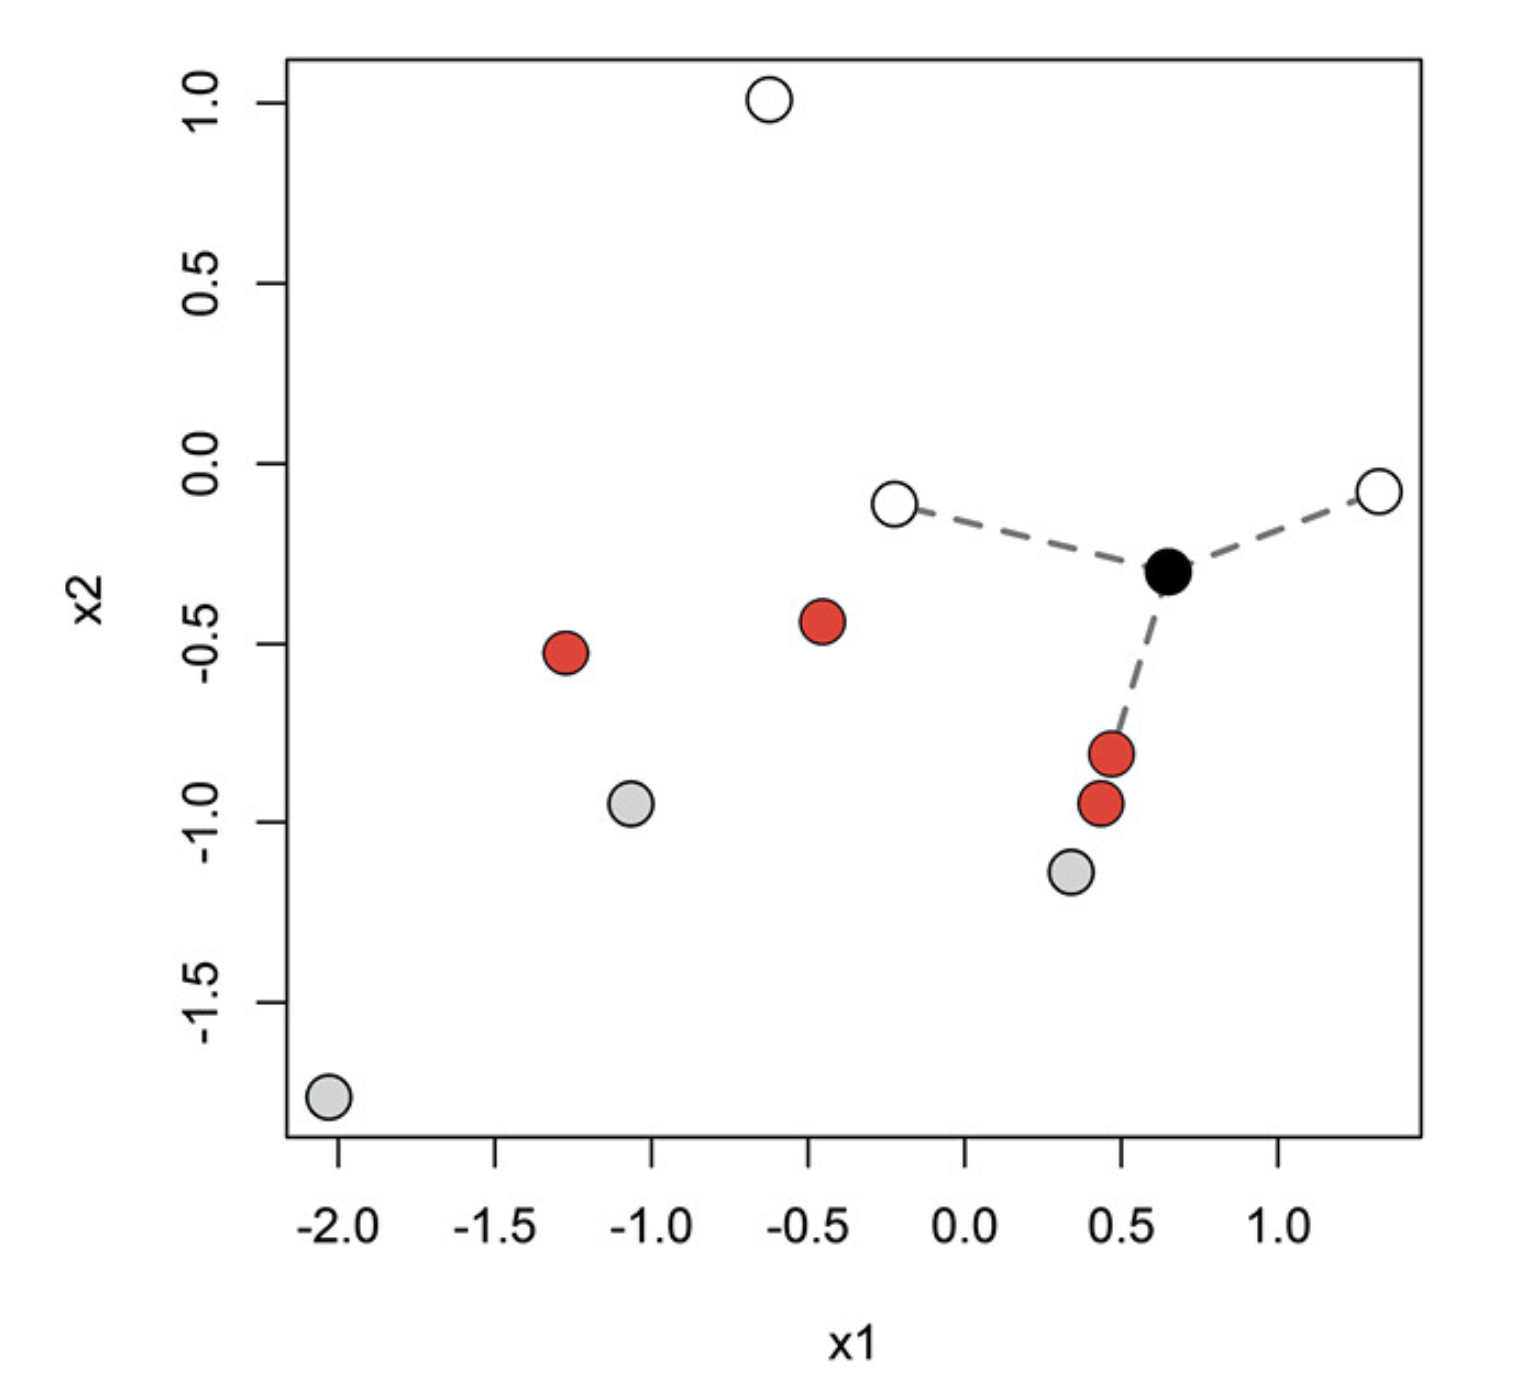
\includegraphics[scale=0.1]{figures/knn}
              \\
              \tiny
              Source: Taddy (2019)
 \end{figure}
\end{column}
\end{columns}
  
\end{frame}


%----------------------------------------------------------------------%
\begin{frame}[fragile]
\frametitle{K-Nearest Neighbors}
\begin{itemize}

  \item There are some major problems with practical implications
  \begin{itemize}
  \item Knn predictions are unstable as a function of $K$
  \medskip
  \item This instability of prediction makes it hard to choose the optimal K and cross validation doesn't work well for KNN
  \medskip
  \item Since prediction for each new $x$ requires a computationally intensive counting, KNN is too expensive to be useful in most big data settings.
  \medskip
  \item KNN is a good idea, but too crude to be useful in practice
  \end{itemize}
\end{itemize}

 \end{frame}

 %----------------------------------------------------------------------%
\subsection{Discriminant Analysis}
%----------------------------------------------------------------------%
%----------------------------------------------------------------------%
\begin{frame}[fragile]
\frametitle{Linear Discriminant Analysis}
\framesubtitle{Reverend Bayes to the rescue: Bayes Theorem}

\bigskip
\begin{align}
Pr (Y=1|X)=\frac{f(X|Y=1)\pi(Y=1)}{m(X)}
\end{align}

\bigskip
with $m(X)$ is the marginal distribution of $X$, i.e.

\begin{align}
m(X)=\int_y f(X|Y=y)\pi(Y=y)dy
\end{align}
\end{frame}
%----------------------------------------------------------------------%
\begin{frame}[fragile]
\frametitle{Linear Discriminant Analysis}
\framesubtitle{Reverend Bayes to the rescue: Bayes Theorem}

Recall that there are two states of nature $y \rightarrow i\in\{0,1\}$
\bigskip
\begin{align}
m(X) &= f(X|Y=1)\pi(Y=1) + f(X|Y=0)\pi(Y=0) 
\end{align}
\medskip
\begin{align}
m(X)     &= f(X|Y=1)\pi(Y=1) + f(X|Y=0)(1-\pi(Y=1))
\end{align}

\end{frame}
%----------------------------------------------------------------------%
\begin{frame}[fragile]
\frametitle{Linear Discriminant Analysis}
\begin{itemize}
  \item This is basically an empirical Bayes approach
  \medskip
  \item We need to estimate $f(X|Y=1)$,  $f(X|Y=0)$ and $\pi(Y=1)$ 
  \medskip
  \begin{itemize}
    \item Let's start by estimating $\pi(Y=1)$. We've done this before
    \medskip
    \begin{align}
    \pi(Y=1) = \frac{\sum_{i=1}^n 1[Y_i=1]}{N}
    \end{align}

      \end{itemize}
\end{itemize}
\end{frame}
%----------------------------------------------------------------------%
\begin{frame}[fragile]
\frametitle{Linear Discriminant Analysis}


\begin{itemize}
    \item Next $f(X|Y=j)$ with $j=0,1$. 
    \medskip
    \begin{itemize}
    \item if we assume one predictor and $X|Y\sim N(\mu_j,\sigma_j)$, the problem boils down to estimating $\mu_j,\sigma_j$
    \medskip
    \item LDA makes it simpler, assumes $\sigma_j=\sigma$ $\forall j$
    \medskip
    \item then partition the sample in two $Y=0$ and $Y=1$, estimate the moments and get $\hat{f}(X|Y=j)$
    \medskip
    \end{itemize}
    \item Plug everything into the Bayes Theorem and you're done
    
\end{itemize}


\end{frame}
%----------------------------------------------------------------------%
\begin{frame}[fragile]
\frametitle{Linear Discriminant Analysis}
\framesubtitle{Extensions}

\begin{itemize}
    \item If we have $k$ predictors?
    \medskip
    \item then $X|Y \sim NM(\mu,\Sigma)$
    \begin{align}
    f(X|Y=j) = \frac{1}{(2\pi)^{k/2}|\Sigma|^{1/2}}exp(-\frac{1}{2}(x-\mu_j)'\Sigma_j(x-\mu_j)
    \end{align}
    \item $\mu_j$ is the vector of the sample means in each partition $j=0,1$
    \medskip
    \item $\Sigma_j$ is the matrix of variance and covariances of each partition $j=0,1$
    
    \end{itemize}
\end{frame}
%----------------------------------------------------------------------%
\begin{frame}[fragile]
\frametitle{Linear Discriminant Analysis}

\begin{itemize}
  \item Why is it called linear?
  \item Note
  \begin{align}
    p>\frac{1}{2} \iff ln(\frac{p}{(1-p)})
  \end{align}
  \item Logit with one predictor
  \begin{align}
  \beta_1 + \beta_2 X
  \end{align}
  \item Classification: in the probability of space
  \item Discrimination: in the space of X
  \item $\beta_1 +\beta_2 X$ is the discrimination function for logit (it is lineal)
\end{itemize}

\end{frame}
%----------------------------------------------------------------------%
\begin{frame}[fragile]
\frametitle{Linear Discriminant Analysis}
\begin{itemize}
  \item LDA?
  \item One predictor with $\sigma_0 = \sigma_1$ (equal variance)
  \begin{align}
  Pr (Y=1|X)=\frac{f(X|Y=1)\pi(Y=1)}{f(X|Y=1)\pi(Y=1) + f(X|Y=0)(1-\pi(Y=1))}
  \end{align}
  \item Then under the equal variance assumption
  \begin{align}
  \frac{Pr (Y=1|X)}{1-Pr(Y=1|X)} &= \frac{f(X|Y=1)\pi(Y=1)}{f(X|Y=0)(1-\pi(Y=1))} \\
                                &= \frac{\pi(Y=1)exp((x-\mu_1)^2)}{(1-\pi(Y=1))exp((x-\mu_0)^2)} 
  \end{align}
\end{itemize}

\end{frame}
%----------------------------------------------------------------------%
\begin{frame}[fragile]
\frametitle{Linear Discriminant Analysis}
\begin{itemize}
  \item Taking logs

\begin{align}
  log \left( \frac{Pr(Y=1|X)}{1-Pr(Y=1|X}\right)  &= log(\frac{\pi(Y=1)}{(1-\pi(Y=1))}+(x-\mu_1)^2-(x-\mu_0)^2 \\
  &= log(\frac{\pi(Y=1)}{(1-\pi(Y=1))}+\mu^2_1-\mu^2_0-2(\mu_1-\mu_0)x \\
  &= \gamma_1 +\gamma_2 X
  \end{align}  
  \item under the assumption of equal variance the discrimination function is linear
  \item Note: logit estimates $\gamma_1$ and $\gamma_2$
\end{itemize}
\end{frame}
%----------------------------------------------------------------------%
\begin{frame}[fragile]
\frametitle{Quadratic Discriminant Analysis}
\begin{itemize}
  \item QDA  assumes diferent variances for the components
\end{itemize}


\begin{figure}[H] \centering
            \captionsetup{justification=centering}
              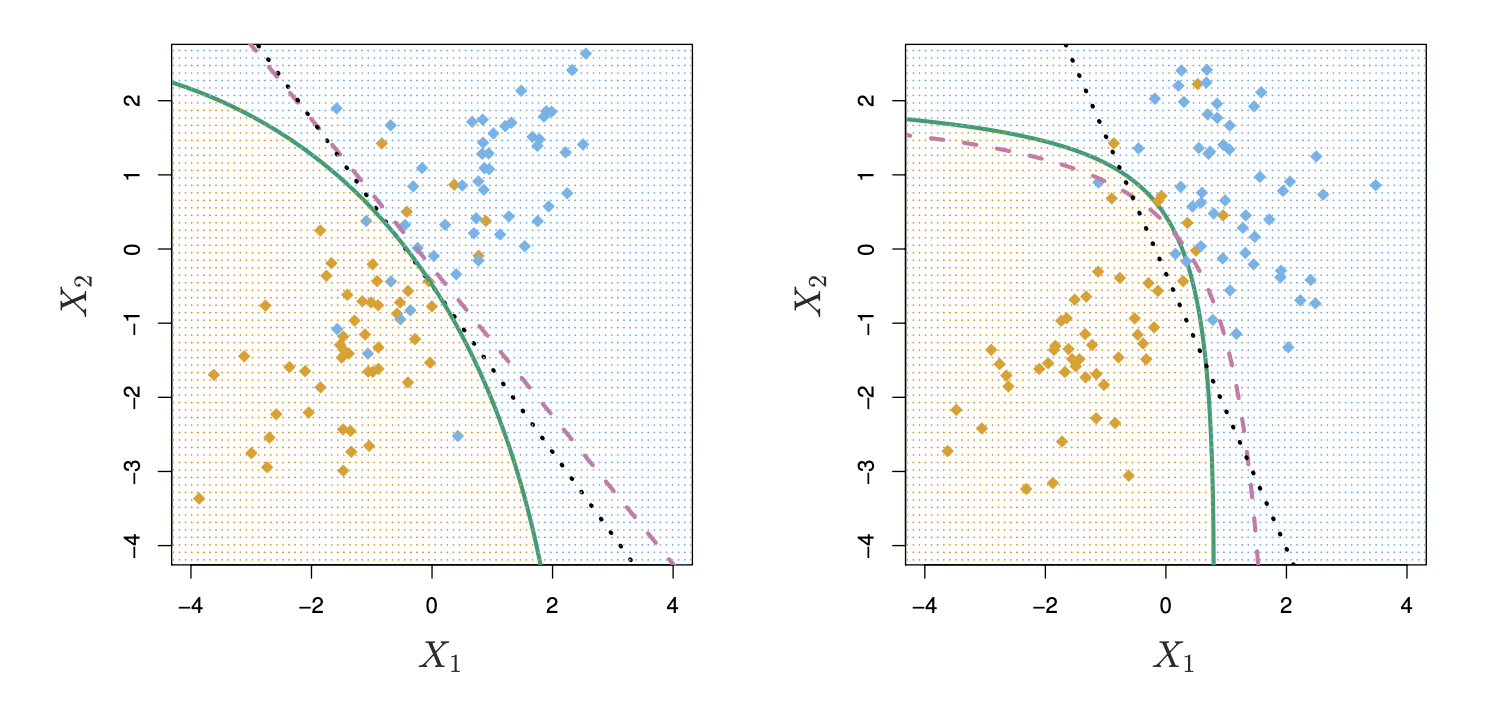
\includegraphics[scale=0.4]{figures/QDA} 
 \end{figure}
\end{frame}
 %----------------------------------------------------------------------%
\subsection{Naive Bayes}
%----------------------------------------------------------------------%
%----------------------------------------------------------------------%
\begin{frame}[fragile]
\frametitle{ Naive Bayes}

\begin{align}
Pr (Y=1|X)=\frac{f(X|Y=1)\pi(Y=1)}{f(X|Y=1)\pi(Y=1) + f(X|Y=0)(1-\pi(Y=1))}
\end{align}

\begin{itemize}
  \item $\pi(Y=1)$
  \item $f(X|Y=1)$
\end{itemize}

\end{frame}

%----------------------------------------------------------------------%
%----------------------------------------------------------------------%
\begin{frame}[fragile]
\frametitle{ Naive Bayes}
\begin{itemize}
  \item NB assumes independence
\begin{align}
  f(X|Y=1)=f(x_1|Y=1) \times \dot \times f(x_k|Y=1)
\end{align}
  
\end{itemize}
\end{frame}
%----------------------------------------------------------------------%
\begin{frame}[fragile]
\frametitle{Example: Default}
\begin{figure}[H] \centering
  \centering
  
\includegraphics[scale=0.35]{figures/baticomputer_meme.jpg}
  \\
  \tiny photo from \url{https://www.dailydot.com/parsec/batman-1966-labels-tumblr-twitter-vine/}
\end{figure}

 \end{frame}


%----------------------------------------------------------------------%
\section{Extra: Kappa statistic}
%----------------------------------------------------------------------%
\begin{frame}[fragile]
\frametitle{Kappa statistic}

\begin{itemize}
  \item Also known as Cohen’s Kappa 
  \item I was originally designed to assess the agreement between two raters (Cohen 1960). 
  \item Kappa takes into account the accuracy that would be generated simply by chance. 


\begin{align}
Kappa = \frac{O - E}{1-E} 
\end{align}

%where O is the observed accuracy and E is the expected accuracy based on the marginal totals of the confusion matrix. 
\item Take on values between -1 and 1; 
\item 0 means  no agreement between the observed and predicted classes, 
\item 1 indicates perfect concordance of the model prediction and the observed classes. 
\item Negative values indicate that the prediction is in the opposite direction of the truth
\end{itemize}
\end{frame}
%----------------------------------------------------------------------%
%----------------------------------------------------------------------%
%----------------------------------------------------------------------%
\end{document}
